% =========================================================================
% Capítulo 0: Repaso
% Álgebra Vectorial y Cálculo Vectorial
% =========================================================================
% Archivo: C0_00_introduccion.tex
% Descripción: Conceptos fundamentales de vectores y cálculo necesarios
%              para el curso de Dinámica de Sistemas Mecánicos
% =========================================================================

\setcounter{chapter}{-1}
\chapter{Repaso}

\section{Conceptos Fundamentales}

\subsection*{Introducción}

En este capítulo repasamos los conceptos esenciales del álgebra vectorial y cálculo vectorial que servirán como base para estudiar dinámica. Los sistemas mecánicos se describen naturalmente mediante vectores, y su evolución temporal se analiza con herramientas del cálculo.

\begin{description}

    \item[Base Orto-normal:] Es una base que tiene la cualidad que todos los vectores que la componen son ortogonales entre ellos (perpendiculares) y que la norma (longitud) de cada uno es unitaria ($\|\vec{e}\|=1$).

    \item[Producto Punto:] También conocido como producto escalar, es muy utilizado para ver la proyección de vectores sobre otros. Si la base es orto-normal el producto punto es $\vec{e}_i\cdot\vec{e}_i=1$ y $\vec{e}_i\cdot\vec{e}_j=0$. Otra fórmula muy útil es $\vec{a}\cdot\vec{b}=\|\vec{a}\|\|\vec{b}\|\cos{(\theta)}$ donde $\theta$ es el ángulo entre ambos vectores.

    \item[Producto Cruz:] También conocido como producto vectorial, que a partir de dos vectores genera un vector perpendicular a ellos (en $\mathbb{R}^3$) cumple la regla de la mano derecha. Se acostumbra a escribir las bases $\{\vec{e}_1,\vec{e}_2,\vec{e}_3\}$ de tal manera que cuando uno calcula el producto cruz de izquierda a derecha el producto cruz entre vectores consecutivos sea el siguiente positivo. Al igual que el producto punto existe otra manera de encontrar el valor del producto cruz: $\vec{a}\times\vec{b}=\|\vec{a}\|\|\vec{b}\|\sin{(\theta)}\vec{n}$ donde $\vec{n}$ es vector de norma 1 perpendicular a ambos.

    \begin{figure}[!ht]
        \centering
        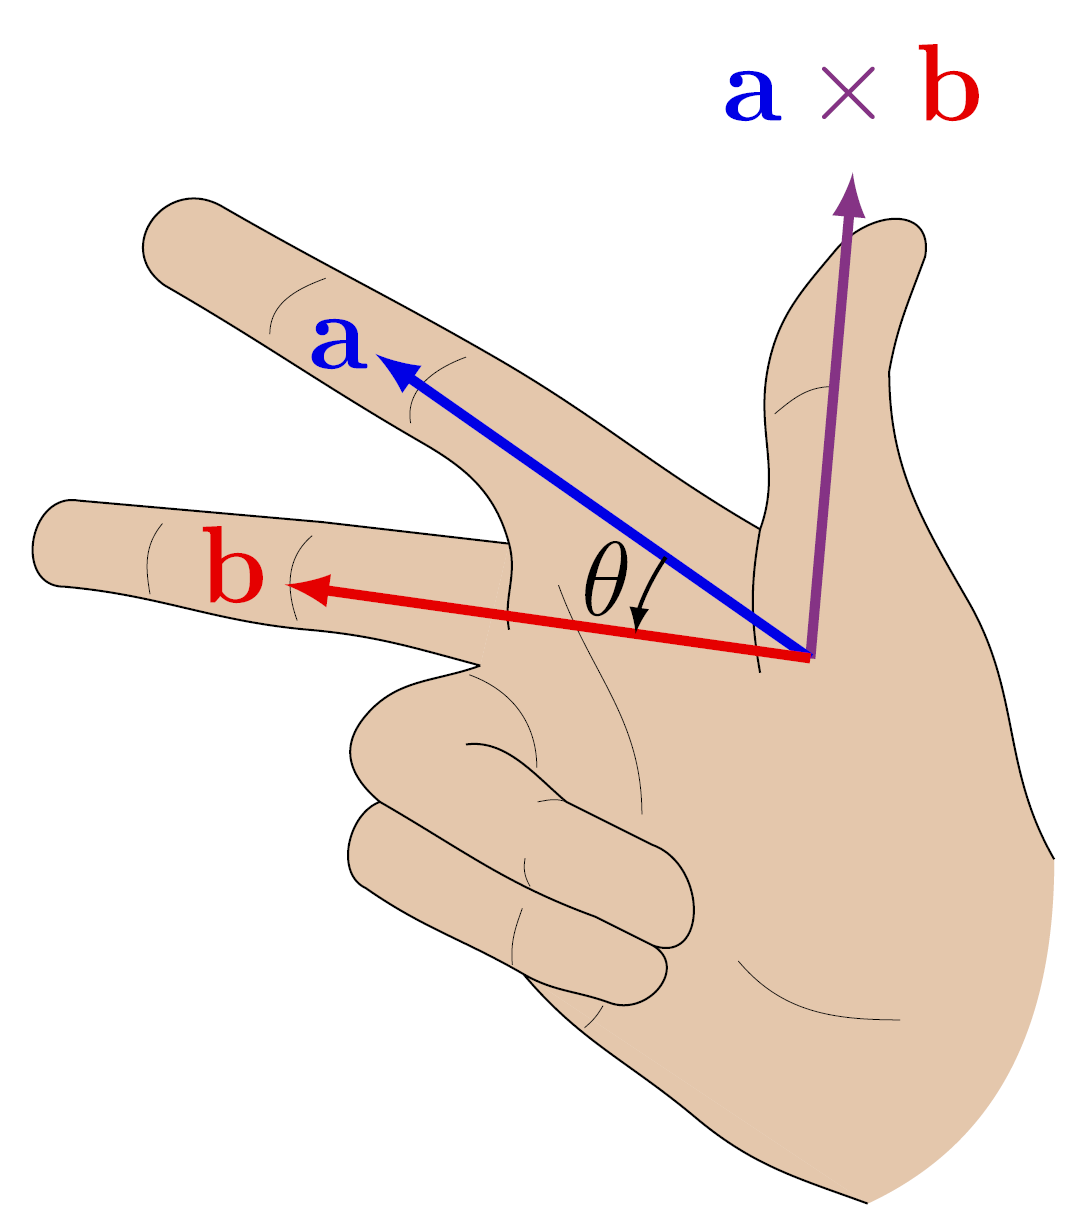
\includegraphics[width=0.15\linewidth]{Contenidos/C0_Repaso/Figuras/RMD1.png}
        \caption{Regla de la mano derecha}
        \label{fig:C0_F01_regla_mano_derecha}
    \end{figure}

    \item[Identidades Vectoriales:] Muy útiles para simplificar ecuaciones de movimiento. El producto triple escalar $\vec{a} \cdot (\vec{b} \times \vec{c})$ representa el volumen del paralelepípedo formado por los vectores. Otra identidad crucial es el doble producto vectorial: $\vec{a} \times (\vec{b} \times \vec{c}) = \vec{b}(\vec{a} \cdot \vec{c}) - \vec{c}(\vec{a} \cdot \vec{b})$.

    \item[Matrices de Rotación:] En $\mathbb{R}^3$, permiten transformar las componentes de un vector entre sistemas de referencia con distinta orientación. Si el sistema $B$ rota respecto al sistema $A$ un ángulo $\theta$ sobre el eje $z$, la matriz de rotación es:
    $$R_{A/B} = \begin{pmatrix} \cos\theta & -\sin\theta & 0 \\ \sin\theta & \cos\theta & 0 \\ 0 & 0 & 1 \end{pmatrix}$$
    Propiedad fundamental: $R^{-1} = R^T$.

    \item[Derivada:] Matemáticamente, es el límite de la razón de cambio de una función respecto a la variación de su variable independiente. Representa la pendiente de la recta tangente a la curva en un punto dado:
    $$f'(x) = \lim_{h \to 0} \frac{f(x+h) - f(x)}{h}$$
    En términos físicos, mide la tasa de variación instantánea de una magnitud.

    \item[Regla de la Cadena:] Es una fórmula para derivar la composición de dos o más funciones. Si $y$ depende de $u$, y $u$ depende de $x$, entonces:
    $$\frac{dy}{dx} = \frac{dy}{du} \cdot \frac{du}{dx}$$
    Es fundamental en dinámica para derivar funciones que dependen implícitamente del tiempo.

    \item[Integral Definida:] Se define como el límite de una suma de áreas de rectángulos (Suma de Riemann) bajo una curva en un intervalo $[a, b]$. Representa la acumulación neta de una cantidad:
    $$\int_{a}^{b} f(x) \, dx = \lim_{n \to \infty} \sum_{i=1}^{n} f(x_i^*) \Delta x$$

    \item[Teorema Fundamental del Cálculo:] Establece la conexión entre la derivación y la integración, indicando que son procesos inversos. Permite calcular integrales mediante la antiderivada $F(x)$:
    $$\int_{a}^{b} f(x) \, dx = F(b) - F(a) \quad \text{donde } F'(x) = f(x)$$

    \item[Gradiente ($\nabla$):] Es un operador vectorial que, aplicado a una función escalar $\phi$, genera un vector cuyas componentes son las derivadas parciales de la función. Indica la dirección de máximo crecimiento de la función:
    $$\nabla \phi = \frac{\partial \phi}{\partial x}\hat{i} + \frac{\partial \phi}{\partial y}\hat{j} + \frac{\partial \phi}{\partial z}\hat{k}$$

    \item[Divergencia ($\nabla \cdot$):] Mide la tendencia de un campo vectorial a originarse o converger en un punto determinado. Es un escalar que resulta del producto punto entre el operador nabla y un vector $\vec{A}$:
    $$\text{div } \vec{A} = \nabla \cdot \vec{A}$$

    \begin{figure}[!ht]
        \centering
        % --- DIVERGENCIA POSITIVA ---
        \tikzset{>=latex}
        \colorlet{veccol}{orange!90!black}
        \colorlet{myblue}{blue!60!black}
        \tikzstyle{vector}=[->,thick,veccol]
        \def\Rad{1.4}
        \def\rad{0.03}
        \def\N{9}

        \begin{tikzpicture}[baseline=(current bounding box.center)]
            \fill[myblue] (0,0) circle (\rad);
            \foreach \i [evaluate={\ang=\i*360/\N;}] in {1,...,\N}{
                \draw[vector] (\ang:0.1*\Rad) --++ (\ang:\Rad);
            }
            \node at (0,-1.5*\Rad) {$\nabla\cdot\vec{v} > 0$};
        \end{tikzpicture}
        \hfill
        % --- DIVERGENCIA NEGATIVA ---
        \begin{tikzpicture}[baseline=(current bounding box.center)]
            \fill[myblue] (0,0) circle (\rad);
            \foreach \i [evaluate={\ang=\i*360/\N;}] in {1,...,\N}{
                \draw[vector] (\ang:1.1*\Rad) -- (\ang:0.1*\Rad);
            }
            \node at (0,-1.5*\Rad) {$\nabla\cdot\vec{v} < 0$};
        \end{tikzpicture}
        \hfill
        % --- DIVERGENCIA CERO ---
        \begin{tikzpicture}[baseline=(current bounding box.center)]
            \foreach \x in {-0.8, 0, 0.8} {
                \foreach \y in {-0.8, 0, 0.8} {
                    \draw[vector] (\x-0.2*\Rad, \y) -- (\x+0.5*\Rad, \y);
                }
            }
            \node at (0,-1.5*\Rad) {$\nabla\cdot\vec{v} = 0$};
        \end{tikzpicture}
        \caption{Representación geométrica de la divergencia}
        \label{fig:C0_F02_divergencia}
    \end{figure}

    \item[Rotor o Rotacional ($\nabla \times$):] Es un operador que mide la tendencia de un campo vectorial a rotar alrededor de un punto. El resultado es un vector:
    $$\text{curl } \vec{A} = \nabla \times \vec{A}$$

    \begin{figure}[!ht]
        \centering
        % --- ROTACIONAL POSITIVO ---
        \tikzset{>=latex}
        \colorlet{veccol}{orange!90!black}
        \colorlet{myblue}{blue!60!black}
        \tikzstyle{vector}=[->,thick,veccol]
        \def\Rad{1.4}
        \def\rad{0.03}
        \def\N{9}

        \begin{tikzpicture}[baseline=(current bounding box.center),scale=0.8]
            \fill[myblue] (0,0) circle (\rad);
            \foreach \i [evaluate={\ang=\i*360/\N;}] in {0,...,\N}{
                \draw[vector] (\ang:\Rad) --++ (\ang+90:0.8*\Rad);
            }
            \node at (0,-1.5*\Rad) {$\nabla\times\vec{v} > 0$};
        \end{tikzpicture}
        \hfill
        % --- ROTACIONAL NEGATIVO ---
        \begin{tikzpicture}[baseline=(current bounding box.center),scale=0.8]
            \fill[myblue] (0,0) circle (\rad);
            \foreach \i [evaluate={\ang=\i*360/\N;}] in {0,...,\N}{
                \draw[vector] (\ang:\Rad) --++ (\ang-90:0.8*\Rad);
            }
            \node at (0,-1.5*\Rad) {$\nabla\times\vec{v} < 0$};
        \end{tikzpicture}
        \hfill
        % --- ROTACIONAL CERO ---
        \begin{tikzpicture}[baseline=(current bounding box.center),scale=0.8]
            \fill[myblue] (0,0) circle (\rad);
            \foreach \i [evaluate={\ang=\i*360/\N;}] in {0,...,\N}{
                \draw[vector] (\ang:0.2*\Rad) -- (\ang:1.2*\Rad);
            }
            \node at (0,-1.5*\Rad) {$\nabla\times\vec{v} = 0$};
        \end{tikzpicture}
        \caption{Rotacional representado mediante vectores tangenciales y radiales}
        \label{fig:C0_F03_rotacional}
    \end{figure}

    \item[Teorema del Transporte:] Sea un vector $\vec{a}$ cualquiera. Su derivada temporal puede ser encontrada como $$\transport{\vec{a}}{A}{B}$$
    
    donde $A$ y $B$ son marcos de referencia.
    Este es un resultado fundamental que conecta las derivadas de un vector en dos sistemas de referencia en rotación relativa.

\end{description}

\newpage

% Incluir secciones teóricas
% =========================================================================
% Capítulo 0 - Sección 1: Álgebra de Vectores
% =========================================================================
\section{Álgebra de Vectores}

Este sección presenta los ejercicios fundamentales de álgebra vectorial,
incluyendo operaciones con bases ortonormales, productos punto y cruz,
e identidades vectoriales clave.

% Incluir ejercicios de Algebra (actualizaremos rutas con cada migración)
\input{Contenidos/Capitulo 0_ Repaso/Ejercicios/Problemas/Algebra/Problema 1}
\input{Contenidos/Capitulo 0_ Repaso/Ejercicios/Problemas/Algebra/Problema 2}
\input{Contenidos/Capitulo 0_ Repaso/Ejercicios/Problemas/Algebra/Problema 3}
\input{Contenidos/Capitulo 0_ Repaso/Ejercicios/Problemas/Algebra/Problema 4}
\input{Contenidos/Capitulo 0_ Repaso/Ejercicios/Problemas/Algebra/Problema 5}
\input{Contenidos/Capitulo 0_ Repaso/Ejercicios/Problemas/Algebra/Problema 6}

\newpage
%% =========================================================================
% Capítulo 0 - Sección 2: Cálculo Vectorial
% =========================================================================
\section{Cálculo Vectorial}

Este sección contiene ejercicios sobre las operaciones de cálculo vectorial:
gradiente, divergencia, rotacional y el teorema del transporte.
Estos conceptos son esenciales para formular las ecuaciones de movimiento.

\subsection{Ejercicios}

\subsection{Problema 1: Derivadas e Integrales Simples}
Resuelva las siguientes operaciones de cálculo básico respecto a una variable $t$ o $x$:

\begin{multicols}{2}
\begin{enumerate}
    \item Halle $\frac{d}{dt} [t^2 \cos(3t)]$.
    \item Halle $\frac{d}{dt} [ \ln(t^2 + 1) e^{-2t} ]$.
    \item Calcule $\int (3t^2 - 5\sin(t)) dt$.
    \item Calcule $\int x e^{x^2} dx$.
    \item Halle $\frac{d}{dt} [ \sqrt{1 + \sin^2(t)} ]$.
    \item Evalúe $\int_0^1 \frac{1}{1+x^2} dx$.
    \item Halle $\frac{d}{dt} [ \arctan(t^2) ]$.
    \item Calcule $\int x^2 \ln(x) dx$.
\end{enumerate}
\end{multicols}
% --- PROBLEMA 2: MULTIVARIABLE (PURO) ---
\subsection{Problema 2: Derivadas Parciales e Integrales Dobles (Cálculo 2)}
Realice los cálculos indicados para funciones de varias variables:

\begin{multicols}{2}
\begin{enumerate}
    \item Sea $f(x,y) = x^3 y^2 + \sin(xy)$, halle $\frac{\partial f}{\partial x}$.
    \item Sea $g(x,y) = e^{x^2+y^2}$, halle $\frac{\partial^2 g}{\partial x \partial y}$.
    \item Evalúe $\int_0^1 \int_0^2 (x + 2y) \, dy \, dx$.
    \item Evalúe $\int_0^\pi \int_0^R r \, dr \, d\theta$.
    \item Halle el gradiente $\nabla \phi$ de $\phi = \sqrt{x^2 + y^2 + z^2}$.
    \item Calcule $\int_0^a \int_0^{a-x} dy \, dx$.
\end{enumerate}
\end{multicols}
% =========================================================================
% Capítulo 0: Repaso
% Tema 02: Cálculo vectorial
% Problema 03: Derivadas de Vectores y Productos
% =========================================================================
\subsubsection{Derivadas de Vectores y Productos}
Considere que $\vec{u}(t)$ y $\vec{v}(t)$ son vectores que dependen del tiempo. Calcule:

\begin{enumerate}
    \item Halle $\frac{d}{dt} (\vec{u} \cdot \vec{v})$.
    \item Halle $\frac{d}{dt} (\vec{u} \times \vec{v})$.
    \item Sea $\vec{r}(t) = \cos(\omega t)\vec{i} + \sin(\omega t)\vec{j} + bt\vec{k}$. Calcule $\dot{\vec{r}}$ y $\ddot{\vec{r}}$.
    \item Si $\vec{v} = \dot{\vec{r}}$, calcule la derivada de la energía cinética escalar: $\frac{d}{dt} (\frac{1}{2} m \vec{v} \cdot \vec{v})$.
\end{enumerate}
% --- SOLUCIÓN ---------------------------------------------------------------
\begin{solucion}{Derivación Vectorial}
\begin{enumerate}
    \item $\frac{d}{dt} (\vec{u} \cdot \vec{v}) = \dot{\vec{u}} \cdot \vec{v} + \vec{u} \cdot \dot{\vec{v}}$.
    \item $\vec{r}(t) = \cos(\omega t)\vec{i} + \sin(\omega t)\vec{j} + bt\vec{k}$. 
    Derivando componente a componente:
    $\dot{\vec{r}} = -\omega\sin(\omega t)\vec{i} + \omega\cos(\omega t)\vec{j} + b\vec{k}$.
    $\ddot{\vec{r}} = -\omega^2\cos(\omega t)\vec{i} - \omega^2\sin(\omega t)\vec{j}$.
    \item $\frac{d}{dt} (\frac{1}{2} m \vec{v} \cdot \vec{v}) = \frac{1}{2} m (\dot{\vec{v}} \cdot \vec{v} + \vec{v} \cdot \dot{\vec{v}}) = m \vec{v} \cdot \dot{\vec{v}} = m \vec{v} \cdot \vec{a} = P$ (Potencia).
\end{enumerate}
\end{solucion}

% --- PROBLEMA 4: BASES INTRÍNSECAS ---
\subsection{Problema 4: Curvas Parametrizadas (Base de Serret-Frenet)}
Para la siguiente curva en el espacio, obtenga los vectores unitarios Tangente ($\hat{T}$), Normal ($\hat{N}$) y Binormal ($\hat{B}$):

$$\vec{r}(s) = \left( a \cos\left(\frac{s}{c}\right), a \sin\left(\frac{s}{c}\right), \frac{b s}{c} \right)$$ 
donde $c = \sqrt{a^2 + b^2}$ y $s$ es el parámetro de longitud de arco.

\begin{enumerate}
    \item Obtenga $\hat{T} = \frac{d\vec{r}}{ds}$.
    \item Obtenga $\hat{N} = \frac{d\hat{T}/ds}{\|d\hat{T}/ds\|}$.
    \item Obtenga $\hat{B} = \hat{T} \times \hat{N}$.
    \item Calcule la curvatura $\kappa = \|\frac{d\hat{T}}{ds}\|$.
\end{enumerate}
% --- PROBLEMA 5: INTEGRALES TRIPLES (APLICADO) ---
\subsection{Problema 5: Distribución de Masa y Volúmenes}
Calcule las siguientes integrales triples sobre los volúmenes indicados (asuma densidad $\rho$ constante):

\begin{enumerate}
    \item Calcule la integral $J = \rho \iiint_V (x^2 + y^2) \, dV$ para un cilindro de radio $R$ y altura $H$ centrado en el eje $z$.
    \item Calcule la integral $P_{xy} = \rho \iiint_V (xy) \, dV$ para un cubo de lado $L$ en el primer octante ($0 \le x,y,z \le L$).
    \item Evalúe $I_0 = \rho \iiint_V (x^2 + y^2 + z^2) \, dV$ para una esfera de radio $R$.
    \item Calcule el volumen de un sólido definido por $x^2 + y^2 \le z \le H$.
\end{enumerate}
% =========================================================================
% Capítulo 0: Repaso
% Tema 02: Cálculo vectorial
% Problema 06: Centros de Masa
% =========================================================================
\subsubsection{Centros de Masa}
El centro de masa ($\vec{r}_{cm}$) representa el punto donde se puede considerar concentrada toda la masa de un sistema.

\begin{enumerate}
    \item Sistema de Partículas: Se tienen tres masas puntuales: $m_1 = 2$ kg en $(1, 0, 0)$, $m_2 = 3$ kg en $(0, 2, 0)$ y $m_3 = 5$ kg en $(0, 0, 2)$. Halle la posición del centro de masa $\vec{r}_{cm}$.
    \item Lámina Semicircular: Calcule la coordenada $\bar{y}$ del centro de masa de una placa plana semicircular de radio $R$ y densidad constante $\rho$, situada en el plano $xy$ sobre el eje $x$ (con el diámetro sobre el eje $x$).
    \item Barra no uniforme: Una barra de longitud $L$ tiene una densidad lineal $\lambda(x) = kx$. Halle la posición $\bar{x}$ de su centro de masa.
\end{enumerate}
% --- SOLUCIÓN ---------------------------------------------------------------
\begin{solucion}{Centro de Masa}
\begin{enumerate}
    \item $\vec{r}_{cm} = \frac{\sum m_i \vec{r}_i}{\sum m_i} = \frac{2(1,0,0) + 3(0,2,0) + 5(0,0,2)}{2+3+5} = \frac{(2, 6, 10)}{10} = (0.2, 0.6, 1.0)$.
    \item $\bar{y} = \frac{1}{M} \iint y \rho dA$. En polares: $y = r\sin\theta$, $dA = r \, dr \, d\theta$.
    $M = \frac{1}{2}\pi R^2 \rho$. 
    $\iint y \rho dA = \rho \int_0^\pi \int_0^R r^2 \sin\theta \, dr \, d\theta = \rho \frac{R^3}{3} [-\cos\theta]_0^\pi = \frac{2\rho R^3}{3}$.
    $\bar{y} = \frac{2\rho R^3 / 3}{\pi R^2 \rho / 2} = \frac{4R}{3\pi}$.
    \item $M = \int_0^L kx \, dx = \frac{1}{2}kL^2$. 
    $\bar{x} = \frac{1}{M} \int_0^L x (kx) dx = \frac{1}{M} \frac{kL^3}{3} = \frac{kL^3/3}{kL^2/2} = \frac{2}{3}L$.
\end{enumerate}
\end{solucion}


\newpage
\subsection{Soluciones}

\subsection{Solucionario: Cálculo}

% ---  1 ---
\begin{sol}[{Cálculo Unidimensional}]
\begin{enumerate}
    \item $\frac{d}{dt} [t^2 \cos(3t)]$: Usando la regla del producto $(uv)' = u'v + uv'$:
    $2t \cos(3t) + t^2 (-\sin(3t) \cdot 3) = 2t\cos(3t) - 3t^2\sin(3t)$.
    
    \item $\frac{d}{dt} [ \ln(t^2 + 1) e^{-2t} ]$: Regla del producto y cadena:
    $\frac{2t}{t^2+1} e^{-2t} + \ln(t^2+1) (-2e^{-2t}) = e^{-2t} \left( \frac{2t}{t^2+1} - 2\ln(t^2+1) \right)$.
    
    \item $\int (3t^2 - 5\sin(t)) dt$: Integración directa:
    $t^3 - 5(-\cos(t)) + C = t^3 + 5\cos(t) + C$.
    
    \item $\int x e^{x^2} dx$: Sustitución $u = x^2$, $du = 2x dx$:
    $\frac{1}{2} \int e^u du = \frac{1}{2} e^{x^2} + C$.
\end{enumerate}
\end{sol}

% ---  2 ---
\begin{sol}[{ Cálculo Multivariable}]
\begin{enumerate}
    \item $\frac{\partial}{\partial x}(x^3 y^2 + \sin(xy))$: Se trata a $y$ como constante:
    $3x^2 y^2 + \cos(xy) \cdot y = 3x^2 y^2 + y\cos(xy)$.
    
    \item $\frac{\partial^2}{\partial x \partial y} (e^{x^2+y^2})$: Primero derivamos respecto a $y$: $\frac{\partial}{\partial y} = 2y e^{x^2+y^2}$. Luego respecto a $x$: $2y (e^{x^2+y^2} \cdot 2x) = 4xy e^{x^2+y^2}$.
    
    \item $\int_0^1 \int_0^2 (x + 2y) \, dy \, dx$: 
    $\int_0^1 [xy + y^2]_0^2 dx = \int_0^1 (2x + 4) dx = [x^2 + 4x]_0^1 = 1 + 4 = 5$.
    
    \item $\int_0^\pi \int_0^R r \, dr \, d\theta$: 
    $\int_0^\pi [\frac{r^2}{2}]_0^R d\theta = \frac{R^2}{2} \int_0^\pi d\theta = \frac{\pi R^2}{2}$.
\end{enumerate}
\end{sol}

% ---  3 ---
\begin{sol}[{ Derivación Vectorial}]
\begin{enumerate}
    \item $\frac{d}{dt} (\vec{u} \cdot \vec{v}) = \dot{\vec{u}} \cdot \vec{v} + \vec{u} \cdot \dot{\vec{v}}$.
    \item $\vec{r}(t) = \cos(\omega t)\vec{i} + \sin(\omega t)\vec{j} + bt\vec{k}$. 
    Derivando componente a componente:
    $\dot{\vec{r}} = -\omega\sin(\omega t)\vec{i} + \omega\cos(\omega t)\vec{j} + b\vec{k}$.
    $\ddot{\vec{r}} = -\omega^2\cos(\omega t)\vec{i} - \omega^2\sin(\omega t)\vec{j}$.
    \item $\frac{d}{dt} (\frac{1}{2} m \vec{v} \cdot \vec{v}) = \frac{1}{2} m (\dot{\vec{v}} \cdot \vec{v} + \vec{v} \cdot \dot{\vec{v}}) = m \vec{v} \cdot \dot{\vec{v}} = m \vec{v} \cdot \vec{a} = P$ (Potencia).
\end{enumerate}
\end{sol}

% ---  4 ---
\begin{sol}[{ Bases Intrínsecas}]
Para $\vec{r}(s) = \left( a \cos(\frac{s}{c}), a \sin(\frac{s}{c}), \frac{bs}{c} \right)$ con $c = \sqrt{a^2+b^2}$:
\begin{enumerate}
    \item $\hat{T} = \frac{d\vec{r}}{ds} = \frac{1}{c} \left( -a\sin(\frac{s}{c}), a\cos(\frac{s}{c}), b \right)$.
    \item $\frac{d\hat{T}}{ds} = \frac{1}{c^2} (-a\cos(\frac{s}{c}), -a\sin(\frac{s}{c}), 0)$. La norma es $\frac{a}{c^2}$.
    $\hat{N} = \frac{d\hat{T}/ds}{a/c^2} = (-\cos(\frac{s}{c}), -\sin(\frac{s}{c}), 0)$.
    \item $\hat{B} = \hat{T} \times \hat{N} = \frac{1}{c} (b\sin(\frac{s}{c}), -b\cos(\frac{s}{c}), a)$.
\end{enumerate}
\end{sol}

% ---  5 ---
\begin{sol}[{ Integrales Triples}]
\begin{enumerate}
    \item $J = \rho \int_0^H \int_0^{2\pi} \int_0^R r^2 (r \, dr \, d\theta \, dz)$: 
    $J = \rho \cdot H \cdot 2\pi \cdot \frac{R^4}{4} = \frac{1}{2} (\rho \pi R^2 H) R^2 = \frac{1}{2} M R^2$.
    \item $P_{xy} = \rho \int_0^L x \, dx \int_0^L y \, dy \int_0^L dz = \rho (\frac{L^2}{2})(\frac{L^2}{2})(L) = \frac{1}{4} \rho L^5 = \frac{1}{4} ML^2$.
\end{enumerate}
\end{sol}

% ---  6 ---
\begin{sol}[{ Centro de Masa}]
\begin{enumerate}
    \item $\vec{r}_{cm} = \frac{\sum m_i \vec{r}_i}{\sum m_i} = \frac{2(1,0,0) + 3(0,2,0) + 5(0,0,2)}{2+3+5} = \frac{(2, 6, 10)}{10} = (0.2, 0.6, 1.0)$.
    \item $\bar{y} = \frac{1}{M} \iint y \rho dA$. En polares: $y = r\sin\theta$, $dA = r \, dr \, d\theta$.
    $M = \frac{1}{2}\pi R^2 \rho$. 
    $\iint y \rho dA = \rho \int_0^\pi \int_0^R r^2 \sin\theta \, dr \, d\theta = \rho \frac{R^3}{3} [-\cos\theta]_0^\pi = \frac{2\rho R^3}{3}$.
    $\bar{y} = \frac{2\rho R^3 / 3}{\pi R^2 \rho / 2} = \frac{4R}{3\pi}$.
    \item $M = \int_0^L kx \, dx = \frac{1}{2}kL^2$. 
    $\bar{x} = \frac{1}{M} \int_0^L x (kx) dx = \frac{1}{M} \frac{kL^3}{3} = \frac{kL^3/3}{kL^2/2} = \frac{2}{3}L$.
\end{enumerate}
\end{sol}

